\subsubsection{Detektion von Baumspitzen}

Auf Basis des generierten CHM erfolgt die Detektion der Baumspitzen. Jede identifizierte Spitze fungiert als eindeutiger Startpunkt für die nachfolgende Segmentierung. Die Präzision dieses Schrittes ist kritisch, da die Anzahl der detektierten Spitzen direkt die finale Anzahl der segmentierten Einzelbäume im Untersuchungsgebiet bestimmt. Bei der Detektion können zwei gegenläufige systematische Fehler auftreten. Während bei einer Übersegmentierung einzelne Äste fälschlicherweise als eigenständige Bäume klassifiziert werden, was die Gesamtzahl künstlich erhöht, führt eine Untersegmentierung zum genauen Gegenteil. Hierbei werden eng zusammenstehende oder ineinandergreifende Kronen als ein einziger Baum erfasst, wodurch kleinere oder unterständige Bäume unberücksichtigt bleiben \cite{fuIndividualTreeSegmentationUAV2024}. Abbildung \ref{fig:seg} veranschaulicht diese beiden Fälle und zeigt ganz links (Abbildung \ref{fig:richtig-seg}), wie eine korrekte Segmentierung aussehen sollte.
\begin{figure}[htbp]
    \centering
    \begin{subfigure}[t]{0.18\columnwidth}
        \centering
        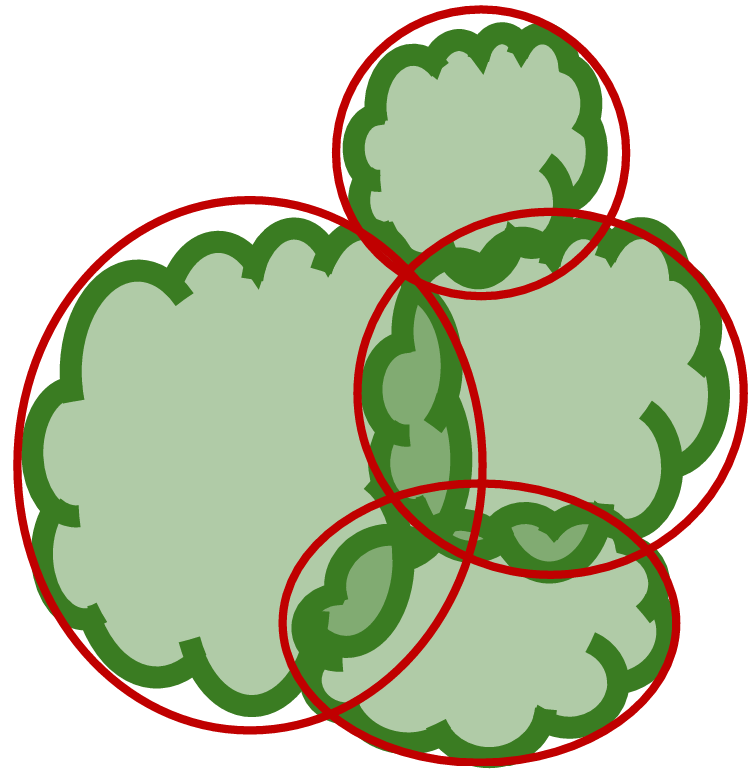
\includegraphics[width=\textwidth]{imgs/richtige-segmentierung.png}
        \caption{Korrekte Segmentierung}
        \label{fig:richtig-seg}
    \end{subfigure}
    \hspace{1,2 cm}
    \begin{subfigure}[t]{0.18\columnwidth}
        \centering
        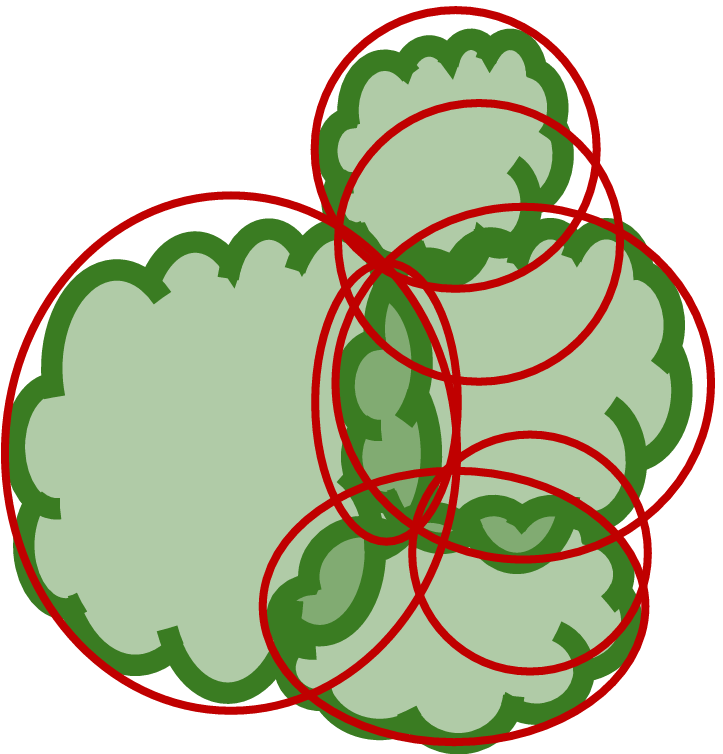
\includegraphics[width=\textwidth]{imgs/uebersegmentierung.png}
        \caption{Übersegmentierung}
        \label{fig:ueberseg}
    \end{subfigure}
    \hspace{1,2 cm}
    \begin{subfigure}[t]{0.18\columnwidth}
        \centering
        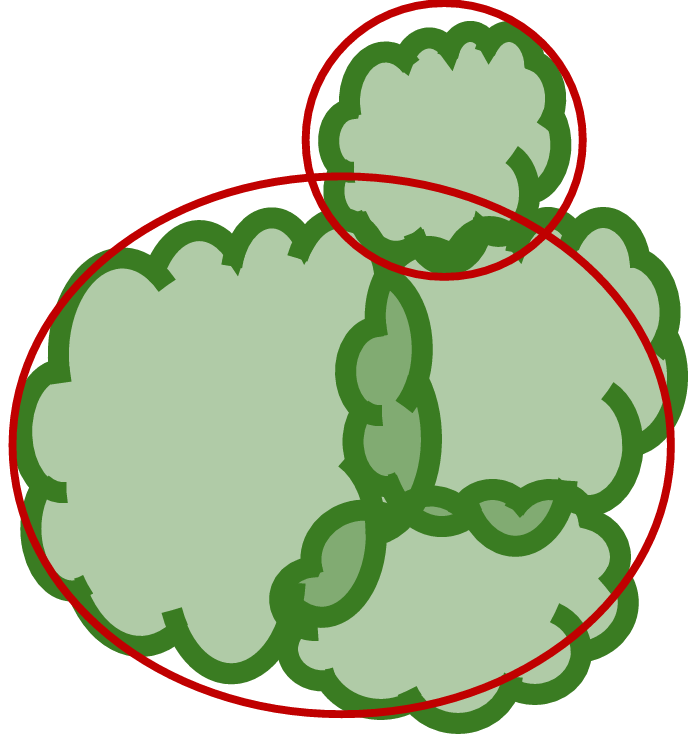
\includegraphics[width=\textwidth]{imgs/untersegmentierung.png}
        \caption{Untersegmentierung}
        \label{fig:unteresg}
    \end{subfigure}
    \caption[Gegenüberstellung von Über- und Untersegmentierung]{Gegenüberstellung von Über- und Untersegmentierung und korrekter Segmentierung}\label{fig:seg}
\end{figure}

Um diese Fehler zu minimieren, wird das CHM zunächst mittels eines Gauß-Filters aus der Bibliothek SciPy geglättet. Dies reduziert das Rauschen, welches durch Höhenvariationen im äußeren Blätterdach verursacht wird. Anschließend wird eine binäre Datenmaske generiert, die alle Pixel unterhalb einer Mindesthöhe von 1,5 m ausschließt, um Bodenvegetation zu eliminieren. Auf dem geglätteten Höhenmodell wird daraufhin innerhalb dieser Maske eine lokale Maximumsuche mit Hilfe der Python-Bibliothek scikit-image durchgeführt. Ein Pixel wird dabei als potenzielles Maximum definiert, wenn es innerhalb einer definierten Nachbarschaft den höchsten Wert aufweist \cite{munzingerMappingUrbanForest2022}.

Da die Gauß-Glättung die realen Baumspitzen geometrisch leicht abflacht, wird für jeden identifizierten Maximum-Kandidaten sowohl die geglättete Höhe ($h_{smooth}$) als auch die Originalhöhe ($h_{raw}$) aus dem ursprünglichen CHM extrahiert. Da biologisch davon ausgegangen wird, dass höhere Bäume breitere Kronen ausbilden, erfordert eine präzise Detektion ein variables statt einem starren Suchfenster. Hierfür wird basierend auf $h_{smooth}$ über eine allometrische Potenzfunktion der theoretisch zu erwartende Kronenradius berechnet. Die empirischen Koeffizienten a und b werden aus dem städtischen Baumkataster kalibriert und durch einen Skalierungsfaktor ($s_{shrink}$) angepasst:
\begin{equation}
    \text{radius} = (a \cdot h_{smooth}^b) \cdot s_{shrink}
    \label{eq:allometric_radius}
\end{equation}
Um biologisch unrealistische Werte bei extremen Baumdimensionen zu vermeiden, wird der berechnete Radius durch feste Schwellwerte begrenzt. 

Im nächsten Schritt werden alle potenziellen Maxima absteigend nach ihrer geglätteten Höhe sortiert, um dominante Bäume im weiteren Prozess zu priorisieren \cite{fuIndividualTreeSegmentationUAV2024}. Zur Eliminierung von Fehlsegmentierungen wird eine iterative Non-Maximum Suppression (\ac{NMS}) angewendet. Hierbei wird ein Kandidat nur dann als finaler Spitzenpunkt akzeptiert, wenn sein euklidischer Abstand zu allen bereits bestätigten, höheren Bäumen einen dynamischen Schwellenwert überschreitet. Dieser minimale Abstand berechnet sich aus dem Kronenradius des größeren, bereits bestätigten Baumes multipliziert mit einem Überlappungsfaktor ($f_{NMS}$):
\begin{equation}
    \text{distanz}_{min} = \text{radius}_{existing} \cdot f_{NMS}
    \label{eq:nms_distance}
\end{equation}
Unterschreitet der Abstand diesen Wert, wird der kleinere Kandidat als Ast oder Nebenkrone verworfen. \cite{yuIndividualTreeSegmentation2024} Die softwaretechnische Zusammenführung dieser adaptiven Radiusermittlung und der anschließenden distanzbasierten Filterung mittels des NMS-Verfahrens ist in Code \ref{lst:adaptiv_radius} dargestellt.

\begin{lstlisting}[label={lst:adaptiv_radius}, caption={[Adaptiver Suchradius zur Baumspitzendetektion]Dynamische Berechnung des adaptiven Suchradius}, breaklines=true, breakatwhitespace=true]
crown_rad = (a * (h_smooth ** b)) * shrink_factor
crown_rad = np.clip(crown_rad, radius_min, radius_max)
peaks.append({"row": row, "col": col, "h_smooth": h_smooth, "h_raw": h_raw, "radius": crown_rad})
peaks = sorted(peaks, key=lambda x: x["h_smooth"], reverse=True)
accepted = []

for cand in peaks:
    keep = True
    for existing in accepted:
        dist = np.sqrt((cand["row"]-existing["row"])**2 + (cand["col"]-existing["col"])**2) * res
        if dist < (existing["radius"] * nms_overlap_factor):
            keep = False
            break
    if keep:
        accepted.append(cand)
\end{lstlisting}

Wie in der Implementierung zu sehen ist, werden die theoretischen Modelle der Formeln \ref{eq:allometric_radius} und \ref{eq:nms_distance} direkt miteinander verzahnt. Der theoretische Kronenradius (\textit{crown\_rad}) wird für jeden identifizierten Maximum-Kandidaten berechnet und zusammen mit den räumlichen Pixel-Koordinaten (\textit{row, col}) in ein Dictionary-Objekt abgelegt. Nach der absteigenden Sortierung der Liste \textit{peaks} durchläuft jeder Punkt die euklidische Distanzprüfung. Ein Baumkandidat wird verworfen, sobald sein mit der Rasterauflösung (\textit{res}) multiplizierter Abstand zu einem bereits akzeptierten Baum dessen individuellen Radius und die Konstante \textit{nms\_overlap\_factor} unterschreitet. Die verbleibenden, validierten Maxima werden unter Verwendung der GeoPandas-Bibliothek als strukturierte Vektordaten aufbereitet und unter Beibehaltung des Koordinatenbezugssystems in einer GPKG-Datei gespeichert.